% ******************************* Thesis Appendix A ****************************
\chapter{Supporting figures to Monte Carlo studies concerning determining interaction times using the effects of diffusion} 

\graphicspath{{Appendix1/Figs/PDF/}{Appendix1/Figs/Raster/}{Appendix1/Figs/Vector/}}

%%%%%%%% The Electron lifetime study
Figure~\ref{fig:DiffLifeStudy_HitFit}, shows how the most probable values of the hit $RMS$ and hit $RMS/Charge$ change as the electron lifetime increases, for hits between 20 and 30 cm from the APAs. Figure~\ref{fig:DiffLifeStudy_CDiff4}, shows how the most probable values of hit $RMS$ changes as drift distance increases for track associated with counter differences of 4, for different values of the electron lifetime. Figure~\ref{fig:DiffLifeStudy_RMS0cm}, shows how the most probable value of hit $RMS$ next to the APAs changes for increasing counter differece. \\ 

\begin{figure}[h!]
  \centering
  \begin{subfigure}{0.45\textwidth}
    \centering
    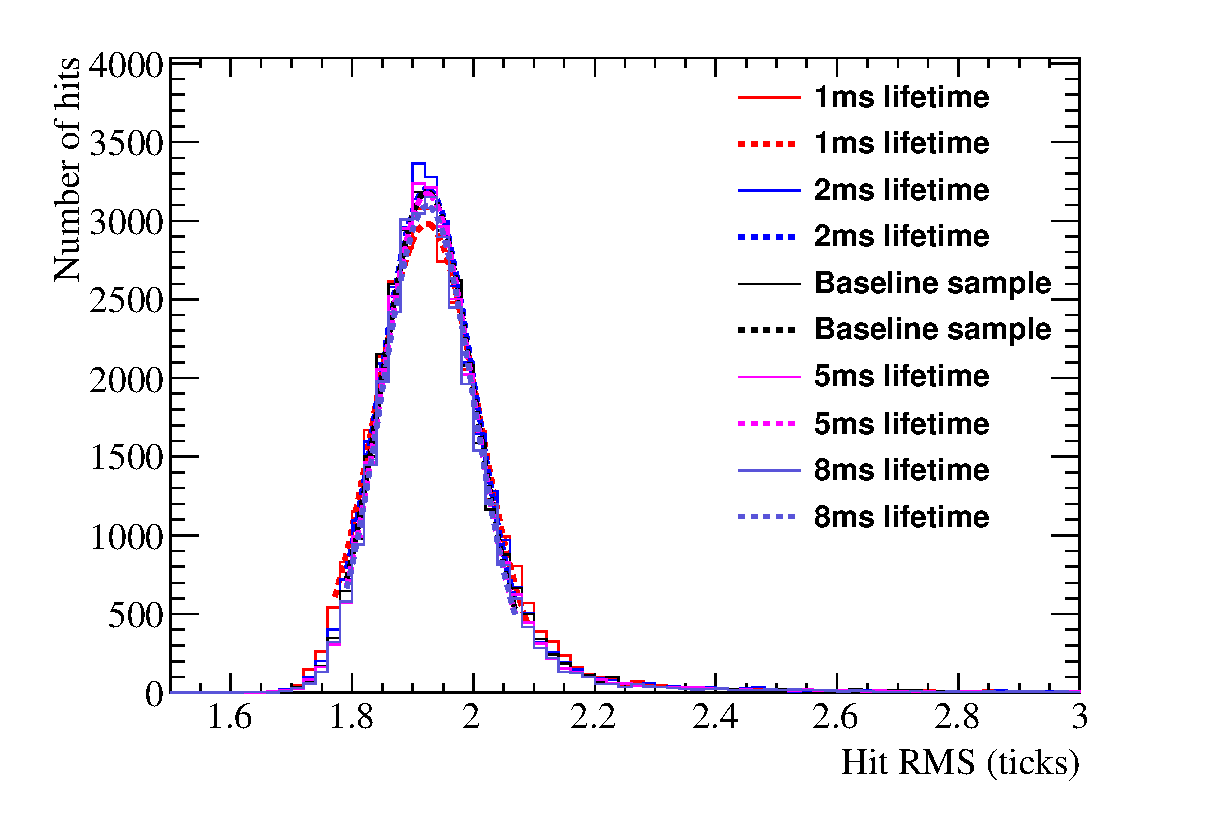
\includegraphics[width=\textwidth]{Canvas_RMS_20cm_ElecLifetime}
    \caption{The most probable hit $RMS$ values for hits between $x =$ 20 cm and $x =$ 30 cm.}
  \end{subfigure}
  \hspace{0.08\textwidth}
  \begin{subfigure}{0.45\textwidth}
    \centering
    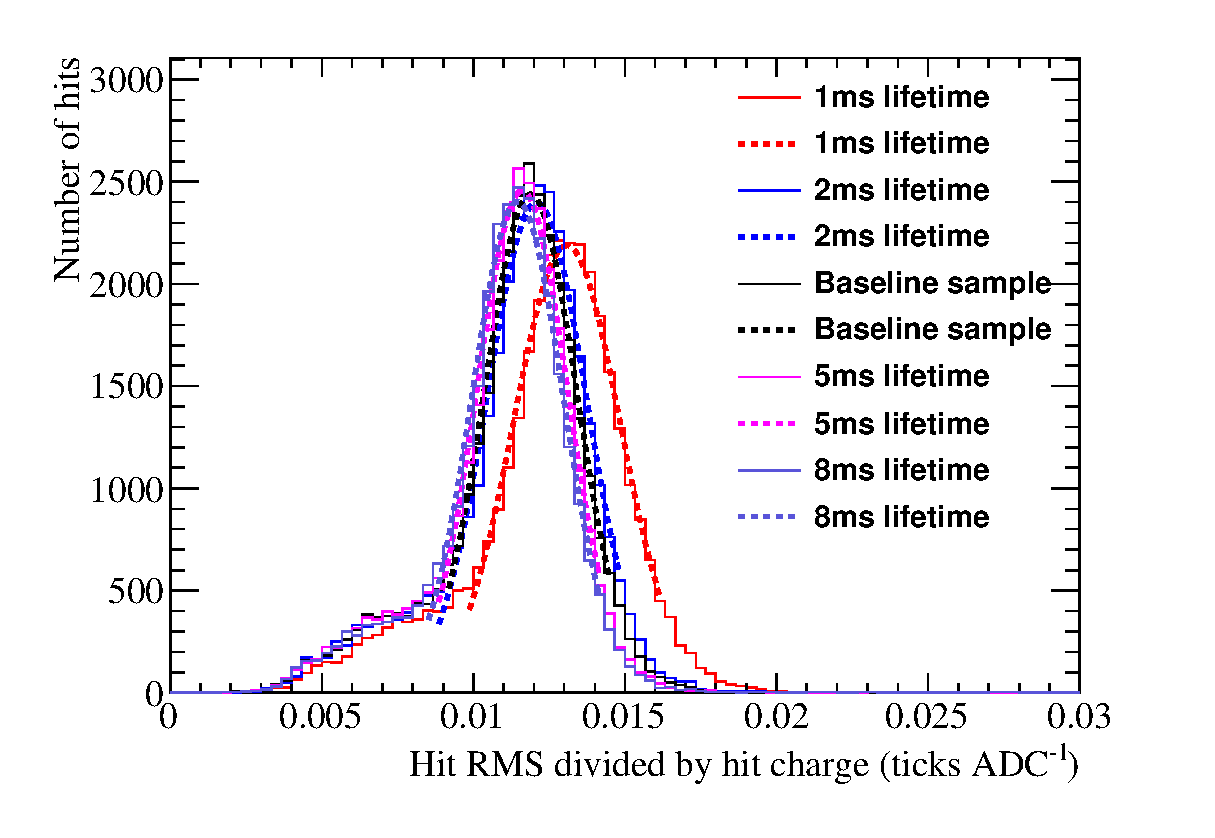
\includegraphics[width=\textwidth]{Canvas_RMS_Q_20cm_ElecLifetime}
    \caption{The most probably hit $RMS/Charge$ values for hits between $x =$ 20 cm and $x =$ 30 cm.}
  \end{subfigure}
  \caption[The most probable values of the hit $RMS$ and hit $RMS/Charge$ distributions for tracks with a counter difference of 4, as the electron lifetime changes]
          {The most probable values of the hit $RMS$ and hit $RMS/Charge$ distributions for hits between $x =$ 20 cm and $x =$ 30 cm, for tracks with a counter difference of 4, as the electron lifetime changes.}
  \label{fig:DiffLifeStudy_HitFit}
\end{figure}

\begin{figure}[h!]
  \centering
  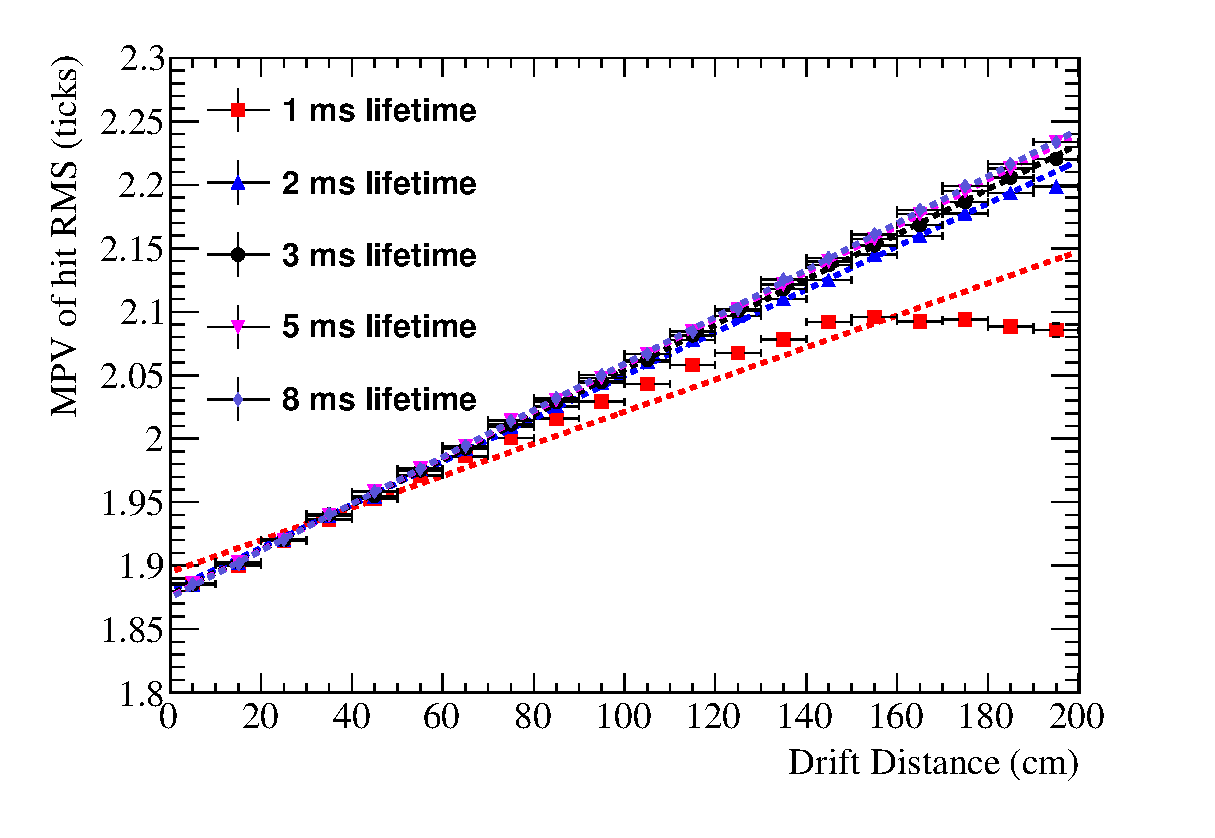
\includegraphics[width=0.6\textwidth]{Canvas_CountDiff4_All_Positions_ElecLifetime}
  \caption[The drift distance dependence of diffusion in the 35 ton dataset and Monte Carlo for coincidences with a counter difference of 4, as the electron lifetime changes]
          {The most probable values of hit $RMS$ as a function of drift distance, for tracks associated with a coincidence that had a counter difference of 4, as the electron lifetime changes.}
  \label{fig:DiffLifeStudy_CDiff4}
\end{figure}

\begin{figure}[h!]
  \centering
  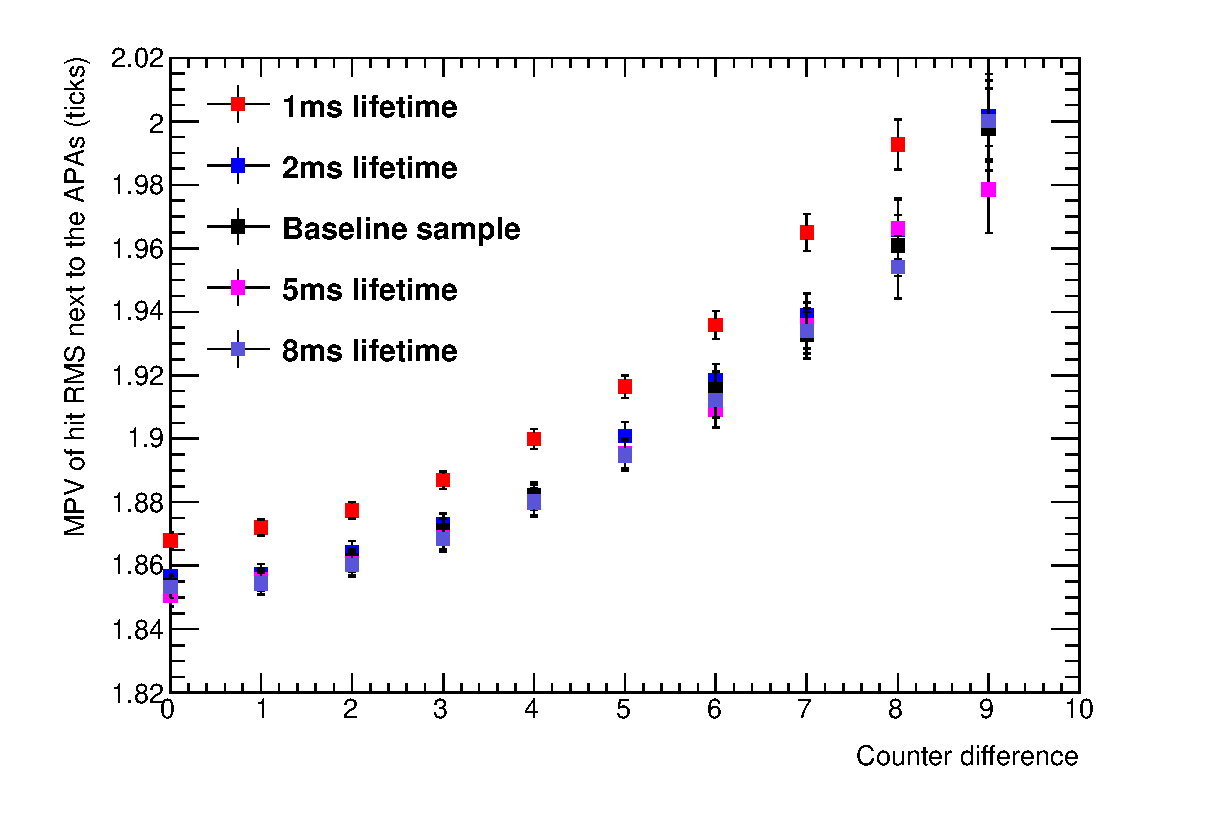
\includegraphics[width=0.6\textwidth]{Canvas_All_Angles_RMS0cm_ElecLifetime}
  \caption[The angular dependence of diffusion in the 35 ton dataset and Monte Carlo for hits within 10 cm of the APAs, as the electron lifetime changes]
          {The most probable values of hit $RMS$ within 10 cm of the APAs, as a function of the counter difference of the coincidence, that the track was associated with, as the electron lifetime changes.}
  \label{fig:DiffLifeStudy_RMS0cm}
\end{figure}

%%%%%%%% The Electric field study
Figure~\ref{fig:DiffElecStudy_HitFit}, shows how the most probable values of the hit $RMS$ and hit $RMS/Charge$ change as the electric field increases, for hits between 20 and 30 cm from the APAs. Figure~\ref{fig:DiffElecStudy_CDiff4}, shows how the most probable values of hit $RMS$ changes as drift distance increases for track associated with counter differences of 4, for different values of the electric field. Figure~\ref{fig:DiffElecStudy_RMS0cm}, shows how the most probable value of hit $RMS$ next to the APAs changes for increasing counter differece. \\

\begin{figure}[h!]
  \centering
  \begin{subfigure}{0.45\textwidth}
    \centering
    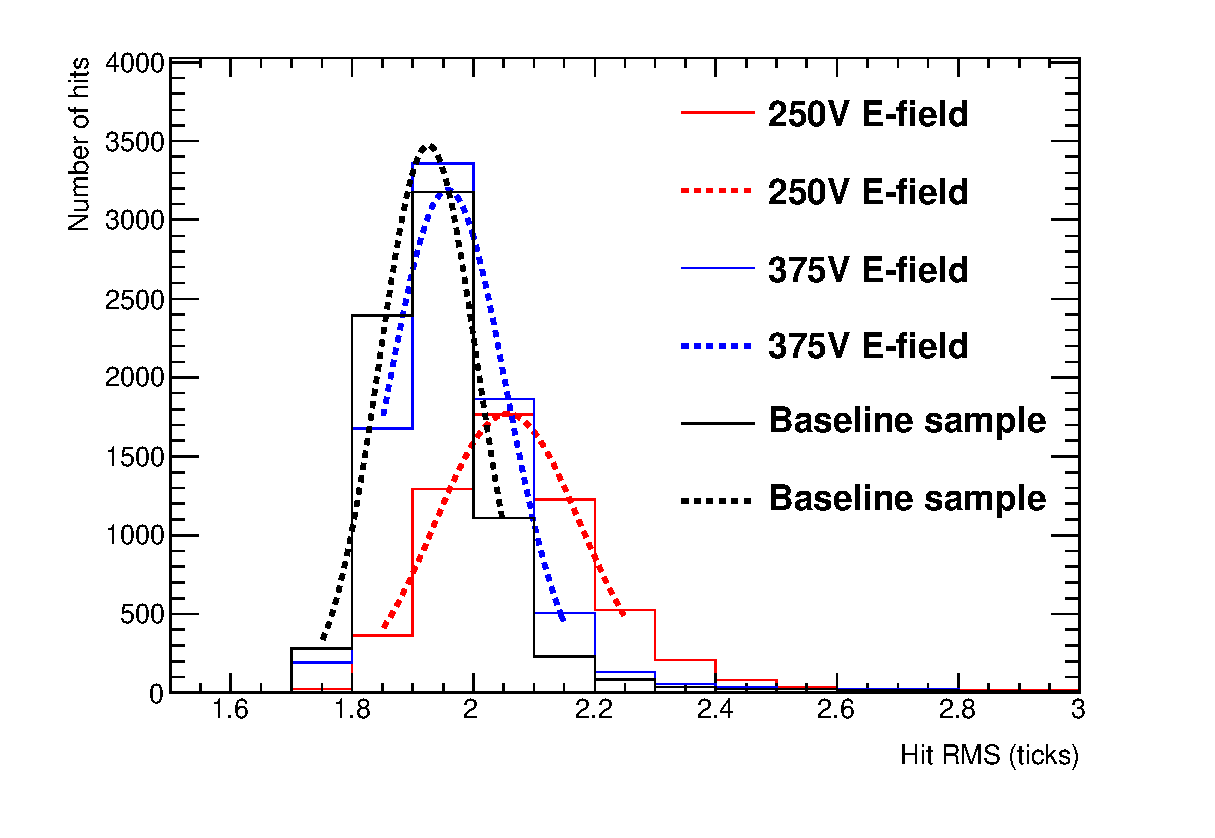
\includegraphics[width=\textwidth]{Canvas_RMS_20cm_ElecField}
    \caption{The most probable hit $RMS$ values for hits between $x =$ 20 cm and $x =$ 30 cm.}
  \end{subfigure}
  \hspace{0.08\textwidth}
  \begin{subfigure}{0.45\textwidth}
    \centering
    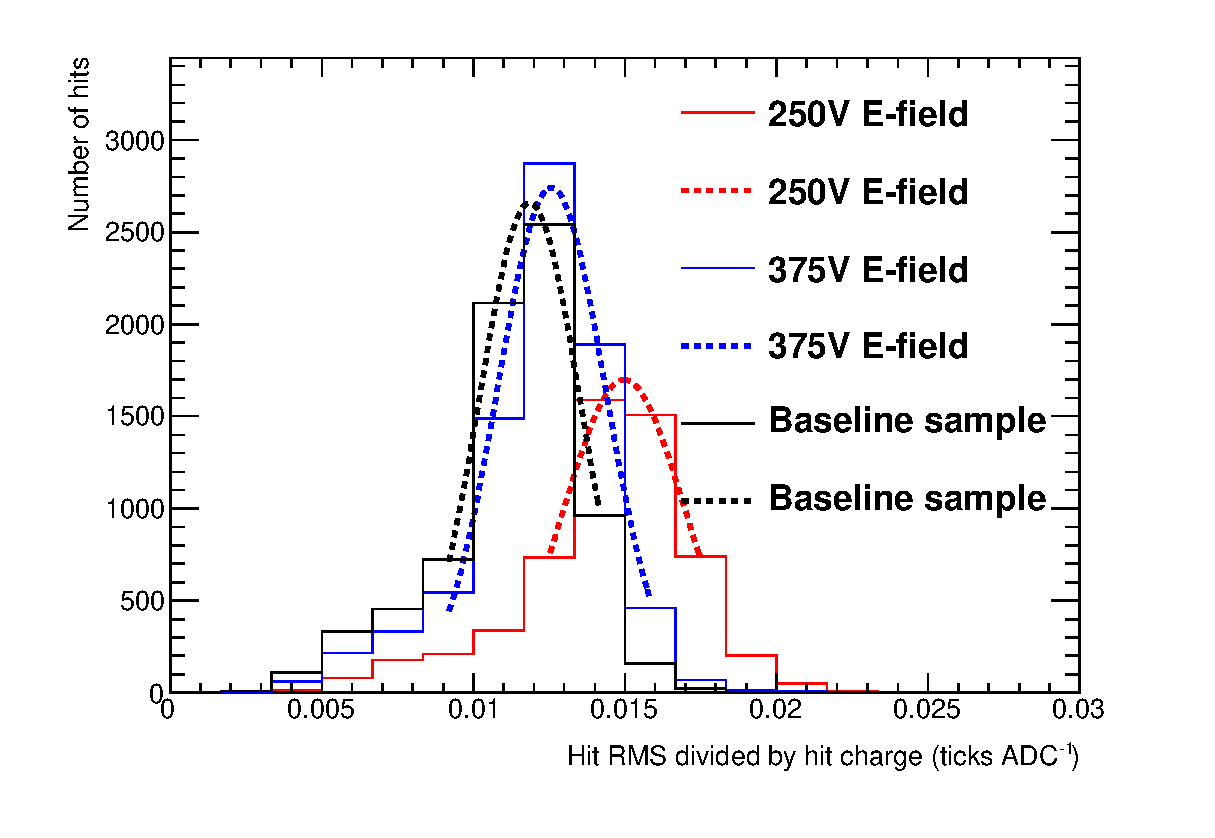
\includegraphics[width=\textwidth]{Canvas_RMS_Q_20cm_ElecField}
    \caption{The most probably hit $RMS/Charge$ values for hits between $x =$ 20 cm and $x =$ 30 cm.}
  \end{subfigure}
  \caption[The most probable values of the hit $RMS$ and hit $RMS/Charge$ distributions for tracks with a counter difference of 4, as the electric field changes]
          {The most probable values of the hit $RMS$ and hit $RMS/Charge$ distributions for hits between $x =$ 20 cm and $x =$ 30 cm, for tracks with a counter difference of 4, as the electric field changes.}
  \label{fig:DiffElecStudy_HitFit}
\end{figure}

\begin{figure}[h!]
  \centering
  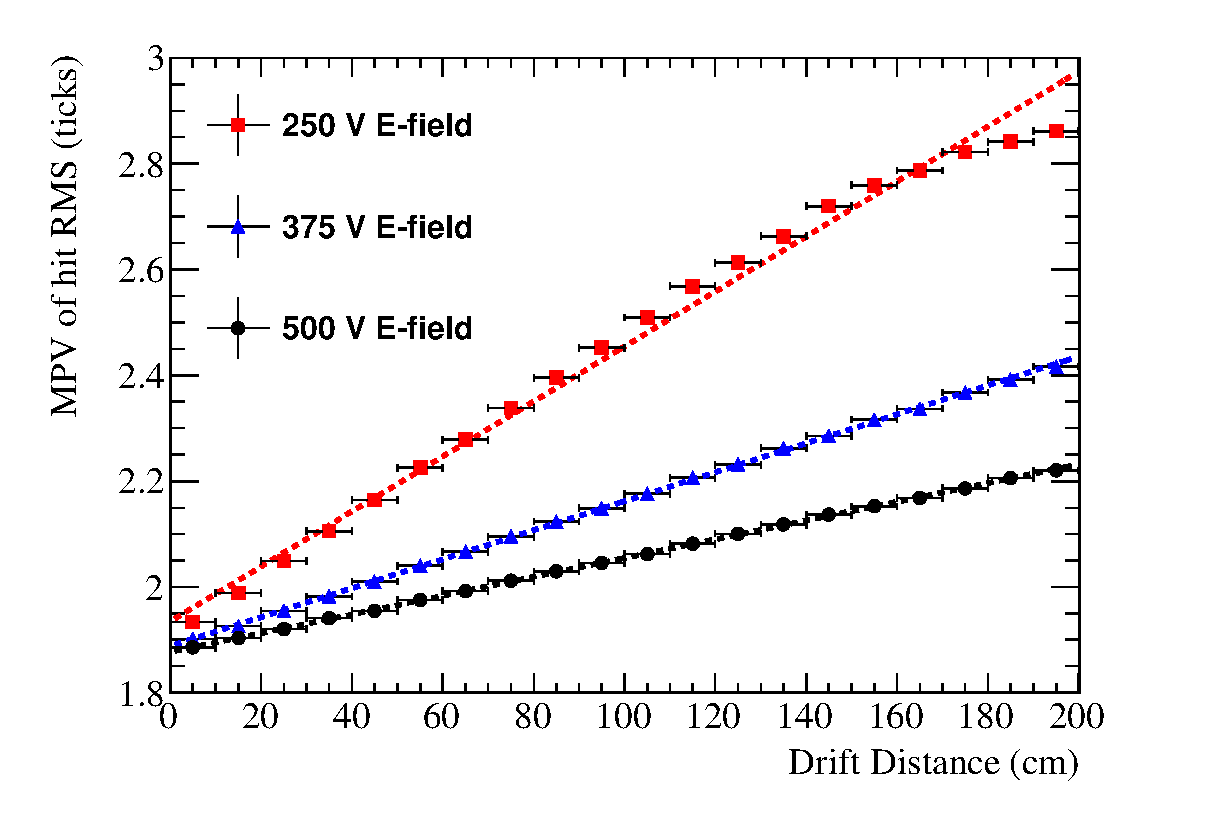
\includegraphics[width=0.6\textwidth]{Canvas_CountDiff4_All_Positions_ElecField}
  \caption[The drift distance dependence of diffusion in the 35 ton dataset and Monte Carlo for coincidences with a counter difference of 4, as the electric field changes]
          {The most probable values of hit $RMS$ as a function of drift distance, for tracks associated with a coincidence that had a counter difference of 4, as the electric field changes.}
  \label{fig:DiffElecStudy_CDiff4}
\end{figure}

\begin{figure}[h!]
  \centering
  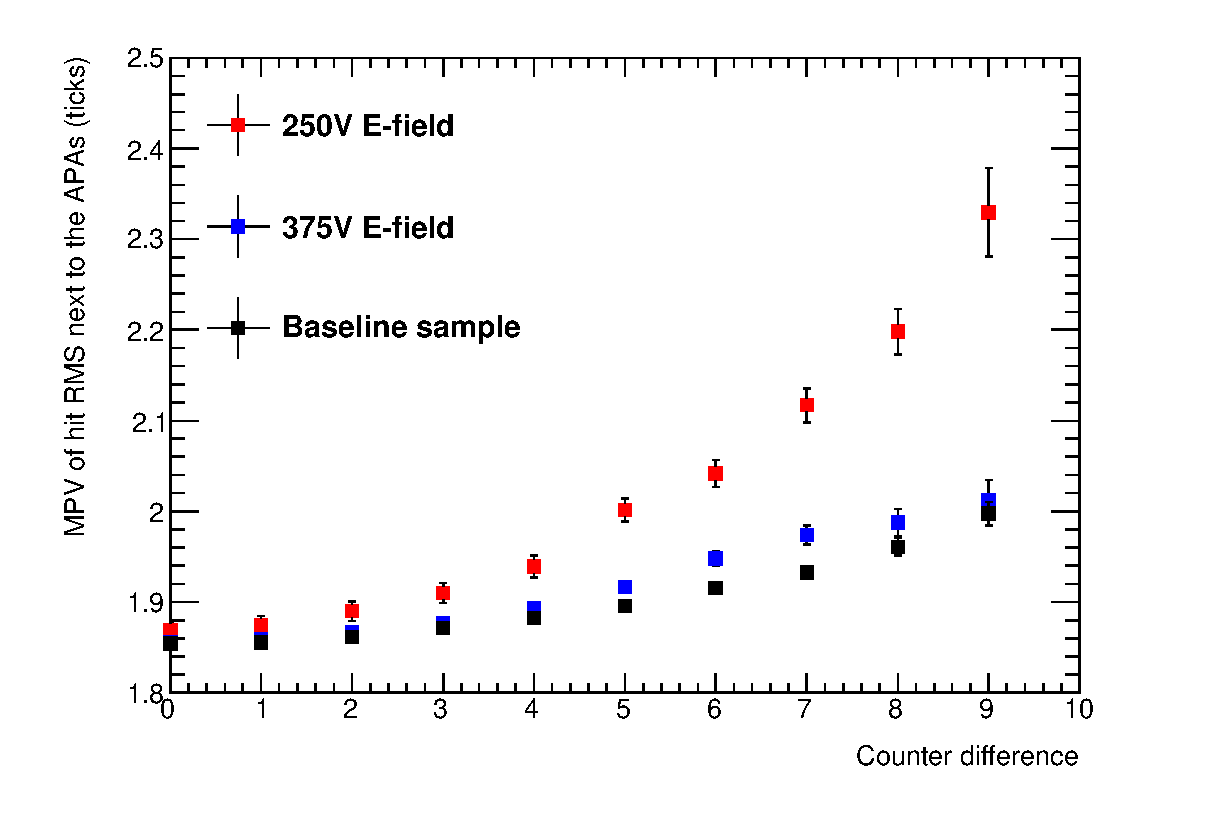
\includegraphics[width=0.6\textwidth]{Canvas_All_Angles_RMS0cm_ElecField}
  \caption[The angular dependence of diffusion in the 35 ton dataset and Monte Carlo for hits within 10 cm of the APAs, as the electric field changes]
          {The most probable values of hit $RMS$ within 10 cm of the APAs, as a function of the counter difference of the coincidence, that the track was associated with, as the electric field changes.}
  \label{fig:DiffElecStudy_RMS0cm}
\end{figure}

%%%%%%%% The diffusion constant study
Figure~\ref{fig:DiffLDiff_HitFit}, shows how the most probable values of the hit $RMS$ and hit $RMS/Charge$ change as the constant of longitudinal diffusion increases, for hits between 20 and 30 cm from the APAs. Figure~\ref{fig:DiffLDiff_CDiff4}, shows how the most probable values of hit $RMS$ changes as drift distance increases for track associated with counter differences of 4, for different values of the constant of longitudinal diffusion. Figure~\ref{fig:DiffLDiff_RMS0cm}, shows how the most probable value of hit $RMS$ next to the APAs changes for increasing counter differece. \\ 

\begin{figure}[h!]
  \centering
  \begin{subfigure}{0.45\textwidth}
    \centering
    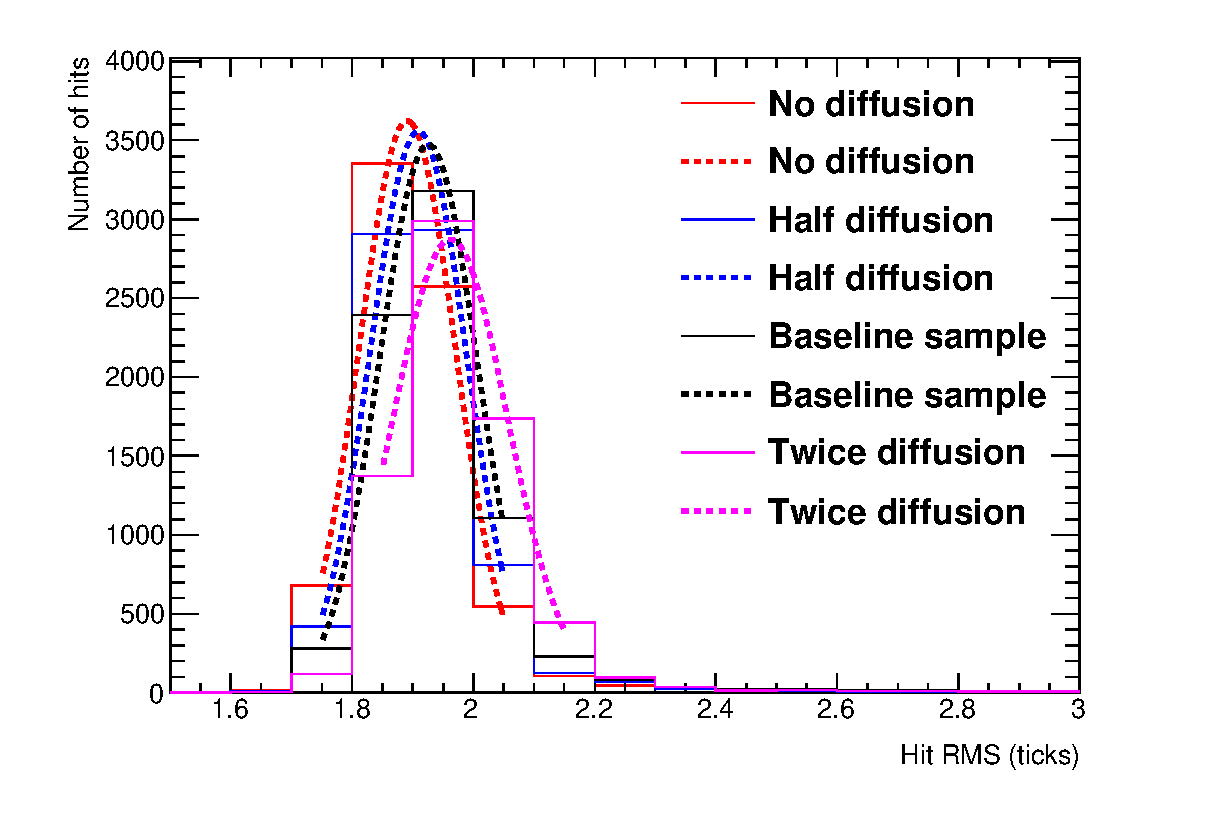
\includegraphics[width=\textwidth]{Canvas_RMS_20cm_Diffusion}
    \caption{The most probable hit $RMS$ values for hits between $x =$ 20 cm and $x =$ 30 cm.}
  \end{subfigure}
  \hspace{0.08\textwidth}
  \begin{subfigure}{0.45\textwidth}
    \centering
    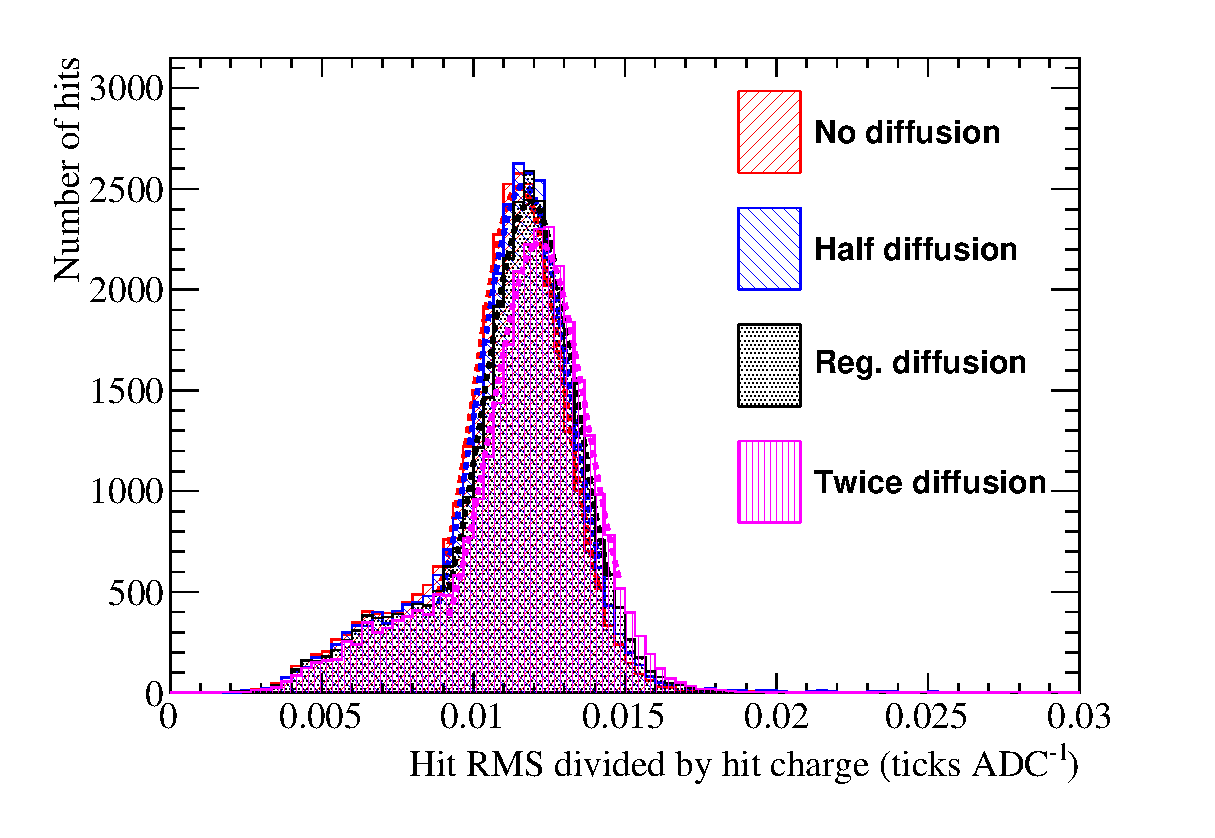
\includegraphics[width=\textwidth]{Canvas_RMS_Q_20cm_Diffusion}
    \caption{The most probably hit $RMS/Charge$ values for hits between $x =$ 20 cm and $x =$ 30 cm.}
  \end{subfigure}
  \caption[The most probable values of the hit $RMS$ and hit $RMS/Charge$ distributions for tracks with a counter difference of 4, as the constant of longitudinal diffusion changes]
          {The most probable values of the hit $RMS$ and hit $RMS/Charge$ distributions for hits between $x =$ 20 cm and $x =$ 30 cm, for tracks with a counter difference of 4, as the constant of longitudinal diffusion changes.}
  \label{fig:DiffLDiff_HitFit}
\end{figure}

\begin{figure}[h!]
  \centering
  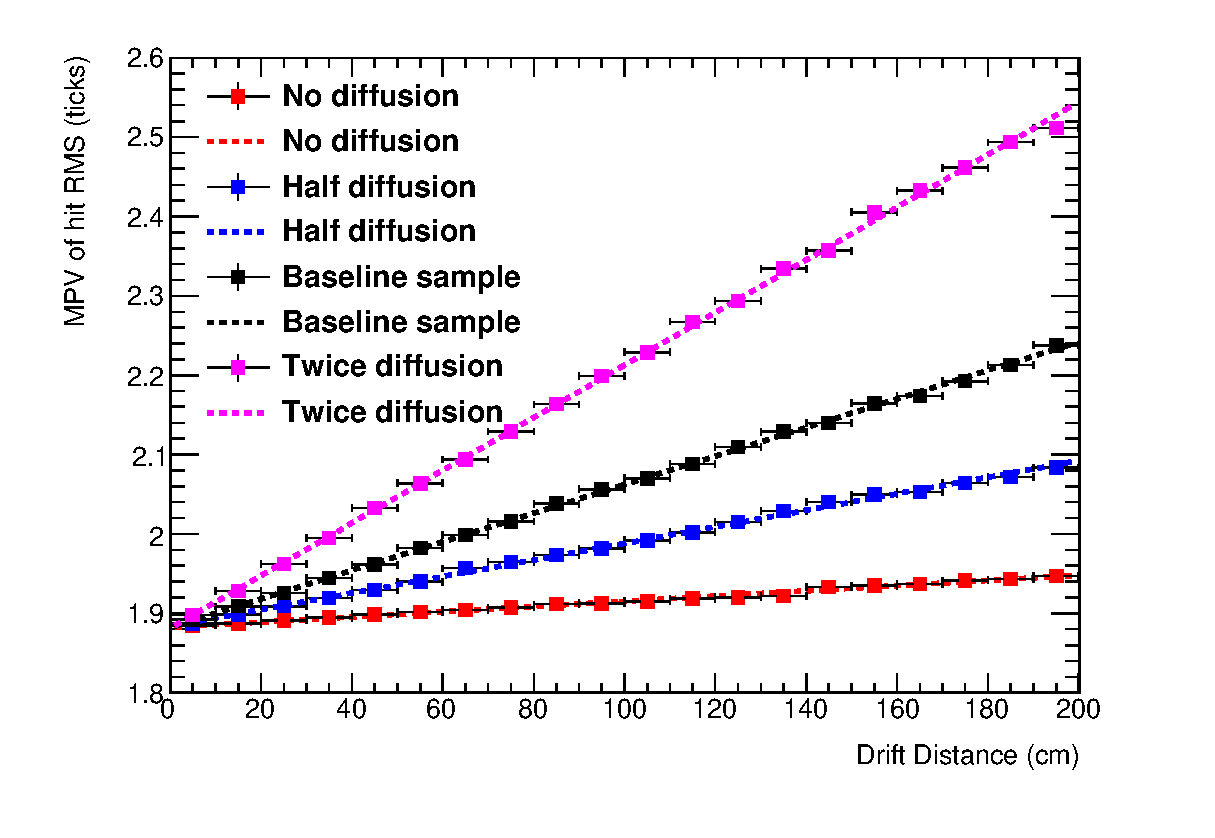
\includegraphics[width=0.6\textwidth]{Canvas_CountDiff4_All_Positions_Diffusion}
  \caption[The drift distance dependence of diffusion in the 35 ton dataset and Monte Carlo for coincidences with a counter difference of 4, as the constant of longitudinal diffusion changes]
          {The most probable values of hit $RMS$ as a function of drift distance, for tracks associated with a coincidence that had a counter difference of 4, as the constant of longitudinal diffusion changes.}
  \label{fig:DiffLDiff_CDiff4}
\end{figure}

\begin{figure}[h!]
  \centering
  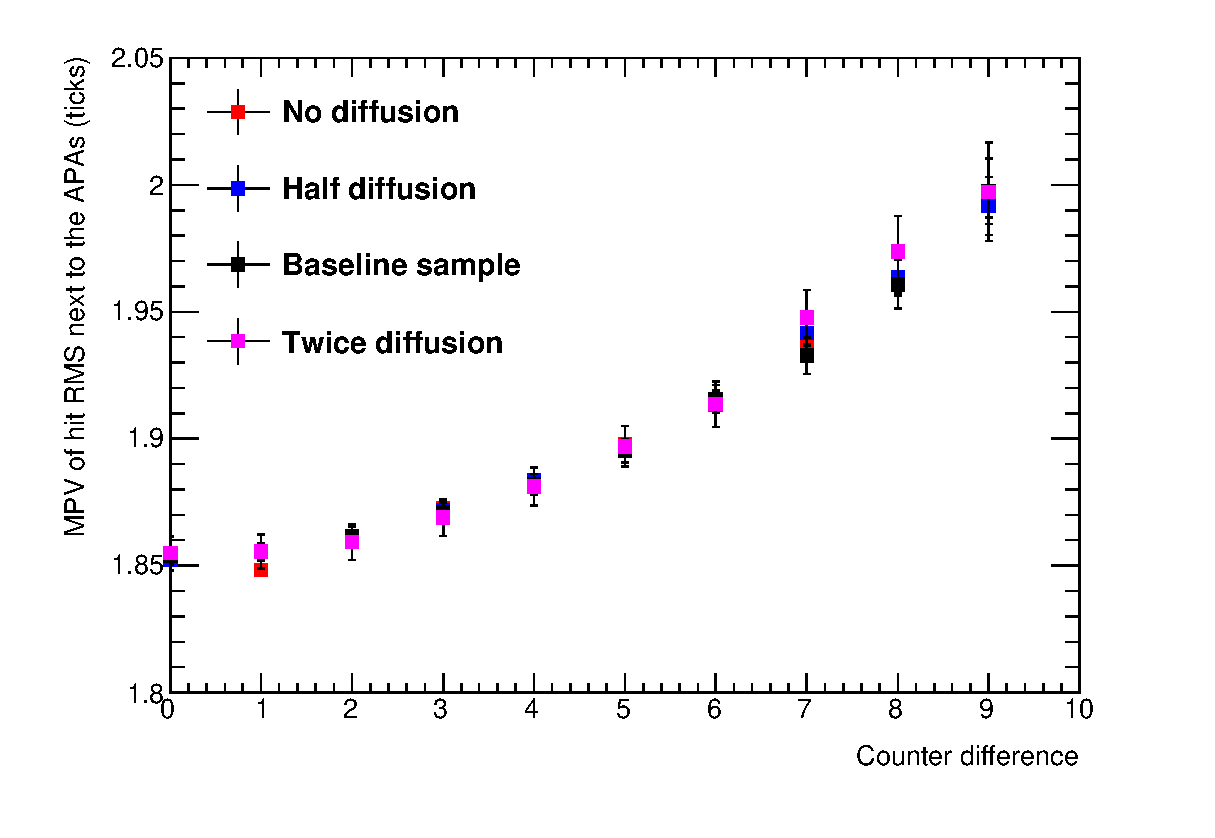
\includegraphics[width=0.6\textwidth]{Canvas_All_Angles_RMS0cm_Diffusion}
  \caption[The angular dependence of diffusion in the 35 ton dataset and Monte Carlo for hits within 10 cm of the APAs, as the constant of longitudinal changes]
          {The most probable values of hit $RMS$ within 10 cm of the APAs, as a function of the counter difference of the coincidence, that the track was associated with, as the constant of longitudinal diffusion changes.}
  \label{fig:DiffLDiff_RMS0cm}
\end{figure}
